%DO NOT MESS AROUND WITH THE CODE ON THIS PAGE UNLESS YOU %REALLY KNOW WHAT YOU ARE DOING
\chapter*{Theory} 
\addcontentsline{toc}{chapter}{Theory}
\section{ Sonar performance prediction } \label{ Sonar performance prediction }

\noindent The basic problem in sonar is to measure some signal (possibly an echo) against a background of noise (or reverberation). So that the signal may be detected above the background, the ratio of the measured signal to the measured background (signal-to-noise ratio) must be at least some minimum value that is determined by the system. The various terms in the sonar equations are called sonar parameters. These parameters may be grouped according to whether they are determined by the equipment, medium, or target. Equipment parameters are source level, detection threshold, directivity index, self-noise level, and array gain (also determined by medium). Medium parameters are transmission loss, ambient noise level, and reverberation level (also determined by equipment). And target parameters are target strength, and target source level. Oceanographic interest in marine acoustics is concentrated mostly in the parameters determined by the medium.

\noindent Sonar may be either active or passive. Active sonar provide their own sound source and listen for echoes as they are reflected from the target which they are trying to detect. Passive sonar have no such source. They are simply listening devises that rely on the target to emit their own noise source (e.g. engine noise from an enemy ship or communication noises from a whale).

\subsection{ Performance parameters } \label{ Performance parameters }
\noindent To assess the capabilities of a sonar system, parameters that measure the performance have to be defined, e.g.
\begin{center}
\begin{tabular}{ |c|c| } 
 \hline
  EL & Echo Level  \\ 
  EE & Echo Excess  \\ 
  SN & Signal to noise ratio  \\ 
  SE & Signal Excess \\
  \hline
\end{tabular}
\end{center}
\noindent Echo level is the intensity of the echo as measured in the water at the hydrophone. Echo excess is obtained by removing the noise from the echo level. The amount by which the signal to noise ratio, SN exceeds the detection threshold, DT, is called the signal excess (SE). If the SE is greater than 0 dB, then the decision is made that the target is present. If the SE is negative, the decision is that the target is not present. The signal to noise ratio, SN is that measured at the output of the receiver, where the decision of whether or not a signal is present is made.

\newpage

\subsection{ Sound propagation related parameters } \label{ Sound propagation related parameters }
\noindent The parameters described in the following sections are transmission loss (\textit{TL}), isotropic noise level (\textit{NL}), bottom reverberation strength (\textit{$RS_B$}), surface reverberation strength (\textit{$RS_S$}) and volume reverberation strength (\textit{$RS_V$}).

\subsubsection{ Transmission loss } \label{ Transmission loss }
\noindent The intensity of an acoustic signal reduces with range. This observed reduction in the acoustic signal with distance from the source is due to the combined effects of spreading and attenuation and is accounted for by the transmission loss term.

\noindent The Transmission loss is given by
\begin{equation}
\textit{TL} = \textnormal{spreading loss} + \textnormal{attenuation} 
\end{equation}
\noindent where \textit{TL} is defined to be 0 dB on a sphere around the source of radius $\textit{r} = 1m.$

\noindent For a constant sound velocity profile and spherical spreading the transmission loss can be determined by
\begin{equation}
\textit{TL(r, z)} = 20 log_{10}{(R)} + \alpha (\textit{R} - 1m)
\end{equation}
\noindent with
\begin{equation}
\textit{R} = \sqrt{ (\textit{r} - \textit{$r_{0}$})^{2} + (\textit{z} - \textit{$z_{0}$})^{2} }
\end{equation}
\noindent where \textit{$r_{0}$}, \textit{$z_{0}$} denote the horizontal and vertical coordinates of the source locations and the receiver position, respectively.

\noindent In case of depth and range dependent cylinder symmetric sound velocity profiles the \textit{TL} can be calculated by
\begin{equation}
\textit{TL(r, z)} = 20 log_{10}{(R)} + 10log_{10}{(\textit{F(r, z))}}  + \alpha (\textit{R} - 1m)
\end{equation}
\noindent where \textit{F(r, z)} denotes the so called focusing factor given by
\begin{equation}
\textit{F(r, z)} = \frac{ \textnormal{ actual spreading at \textit{r, z}}}{ spherical spreading at \textit{r, z}}
\end{equation}

\subsubsection{ Isotropic noise level } \label{ Isotropic noise level }
\noindent This is an essentially a steady state, isotropic (equal in all directions) sound which is generated by amongst other things wind, waves, biological activity and shipping. The isotropic noise level \textit{NL(f,$v_w$,r,s,$v_v$)} describes for particular \textit{$v_w$}, \textit{r}, \textit{s} and \textit{$v_v$} the noise power within a 1Hz band around frequency \textit{f}.

\noindent Thus, assuming \textit{NL} approximately white over the frequency band \textit{B} of interest, the noise level is given by
\begin{equation}
\textit{$NL_B$} = \textit{NL(f,$v_w$,r,s,$v_v$)} + 10log_{10}{\textit{B}}
\end{equation}

\subsubsection{ Bottom reverberation strength } \label{ Bottom reverberation strength }
\noindent The bottom reverberation coefficient \textit{$RS_{B}(f,bt,\beta)$} describes the reverberation strength of an insonified area of $1 m^2.$

\noindent With 
\begin{center}
\begin{tabular}{ |c|c| } 
 \hline
  \textit{c} & sound speed  \\ 
  $\uptau$ & pulse length \\ 
  $2 \theta_{h}$  & min($2\theta_{h,T}, 2\theta_{h,R}$)  \\ 
  $2\theta_{h,T}$ &  horizontal $3 dB$ beam width of transmitter \\
  $2\theta_{h,R}$  & horizontal $3 dB$ beam width of receiver \\ 
  \textit{$r_0/ z_0$} & coordinates of transmitter/ receiver configuration \\
  \textit{r/ z} & coordinates of a particular point on the sea floor\\
  \hline
\end{tabular}
\end{center}

\noindent The bottom reverberation strength can be determined for given \textit{f} and \textit{bt} as a function of $\beta$ by
\begin{equation}
\textit{$RS_B$} = \textit{$S_{B}(f,bt,\beta)$} + 10 log_{10}{(A_B)}
\end{equation}
\noindent where \textit{$A_B$} denotes the insonified bottom area.
\begin{equation}
\textit{$A_B$} = 2 \theta_{h} R \frac{ c \uptau }{ 2 cos{\beta}}
\end{equation}
\noindent with
\begin{equation}
\textit{R} = \sqrt{ (\textit{r} - \textit{$r_{0}$})^{2} + (\textit{z} - \textit{$z_{0}$})^{2} }
\end{equation}

\begin{figure}[H]
\centering
{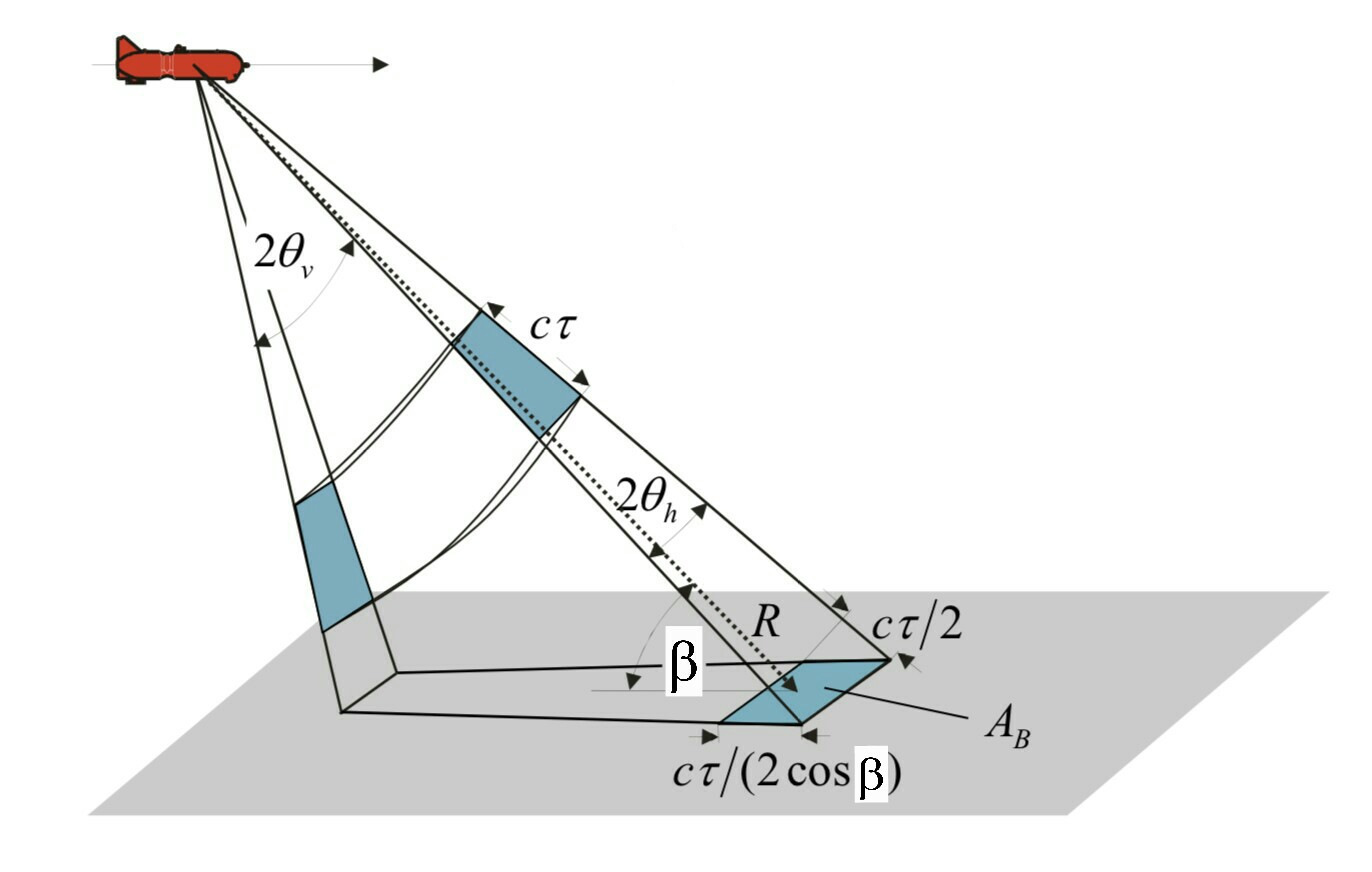
\includegraphics[scale=0.16]{theory1.jpg}}
\caption{Surface reverberation versus grazing angle for frequency dependency}
\end{figure}

\subsubsection{ Surface reverberation strength } \label{ Surface reverberation strength }
\noindent Analog to the bottom reverberation strength, the surface reverberation strength is provided by
\begin{equation}
\textit{$RS_S$} = \textit{$S_{S}(f,bt,\beta)$} + 10 log_{10}{(A_S)}
\end{equation}
\noindent where \textit{$A_S$} denotes the insonified sea surface area.
\begin{equation}
\textit{$A_S$} = 2 \theta_{h} \sqrt{ (\textit{r} - \textit{$r_{0}$})^{2} + (\textit{z} - \textit{$z_{0}$})^{2} } \frac{ c \uptau }{ 2 cos{\beta}}
\end{equation}
\noindent With
\begin{center}
\begin{tabular}{ |c|c| } 
 \hline
  \textit{c} & sound speed  \\ 
  $\uptau$ & pulse length \\ 
  $2 \theta_{h}$  & min($2\theta_{h,T}, 2\theta_{h,R}$)  \\ 
  $2\theta_{h,T}$ &  horizontal $3 dB$ beam width of transmitter \\
  $2\theta_{h,R}$  & horizontal $3 dB$ beam width of receiver \\ 
  \textit{$r_0/ z_0$} & coordinates of transmitter/ receiver configuration \\
  \textit{r/ z} & coordinates of a particular point on the sea surface\\
  \hline
\end{tabular}
\end{center}

\subsubsection{ Volume reverberation strength } \label{ Volume reverberation strength }
\noindent The volume reverberation coefficient \textit{$RS_{V}(f,bt,\beta)$} describes the reverberation strength of an insonified area of $1 m^3.$ Thus, the volume reverberation strength can be calculated by
\begin{equation}
\textit{$RS_V$} = \textit{$S_{V}(S_p, f)$} + 10 log_{10}{(V)}
\end{equation}
\noindent where \textit{V} denotes the insonified volume (isovelocity).
\begin{equation}
\textit{V} = \frac{ c \uptau }{ 2 cos{\beta}} 2 \theta_{h} 2 \theta_{v} R^{2}
\end{equation}
\noindent and
\begin{equation}
\textit{R} = \sqrt{ (\textit{r} - \textit{$r_{0}$})^{2} + (\textit{z} - \textit{$z_{0}$})^{2} }
\end{equation}
\noindent With
\begin{center}
\begin{tabular}{ |c|c| } 
 \hline
  \textit{c} & sound speed  \\ 
  $\uptau$ & pulse length \\ 
  $2 \theta_{h}$ / $2 \theta_{v}$ & min($2\theta_{h,T}, 2\theta_{h,R}$) / min($2\theta_{v,T}, 2\theta_{v,R}$)  \\ 
  $2\theta_{h,T}$ / $2\theta_{v,T}$ &  horizontal / vertical $3 dB$ beam width of transmitter \\
  $2\theta_{h,R}$ / $2\theta_{v,R}$ & horizontal / vertical $3 dB$ beam width of receiver \\ 
  \textit{$r_0/ z_0$} & coordinates of transmitter/ receiver configuration \\
  \textit{r/ z} & coordinates of a particular point on water volume \\
  \hline
\end{tabular}
\end{center}

\begin{figure}[H]
\centering
{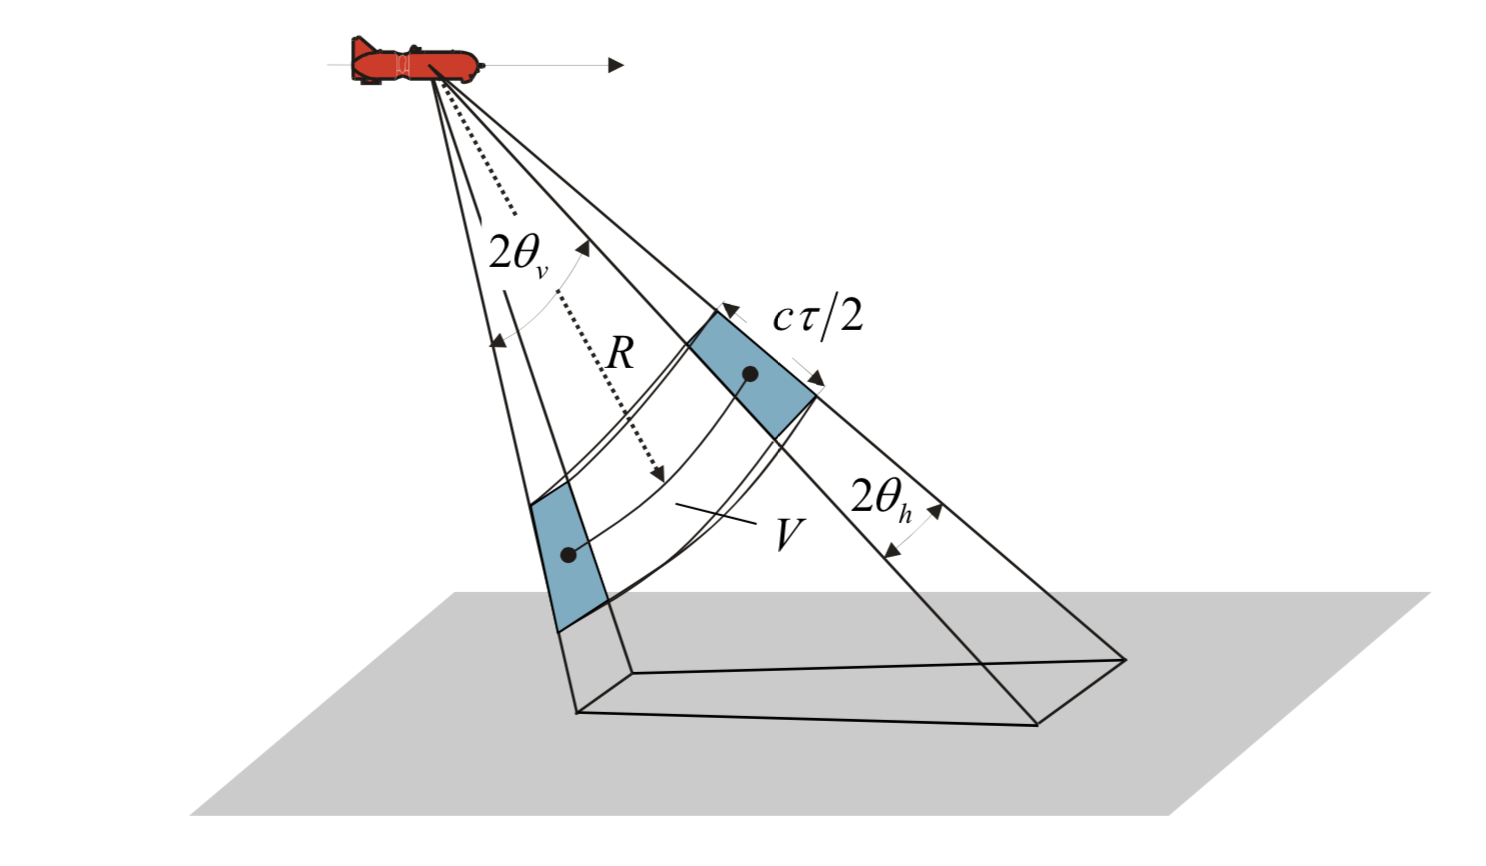
\includegraphics[scale=0.40]{theory2.png}}
\caption{Surface reverberation versus grazing angle for frequency dependency}
\end{figure}

\newpage

\subsection{ Sonar equation } \label{ Sonar equation}
\noindent To determine the aforementioned reverberation levels the following parameters have to be specified.
\begin{center}
\begin{tabular}{ |c|c| } 
 \hline
 \multicolumn{2}{|c|}{Environmental Parameters} \\
 \hline
  \textit{bt} & Bottom type  \\ 
  \textit{$v_w$} & Wind speed  \\ 
  \textit{S} & Salinity  \\ 
  \textit{T} & Water temperature \\
  \textit{c} & Sound speed profile \\
  \hline
\end{tabular}
\end{center}

\noindent Source level is the ratio of the source intensity to a reference intensity, converted to dB. The reference intensity is the intensity of a sound wave having a root mean square (rms) pressure of $1 \mu Pa.$Directivity index is the amount by which the antenna array has to reject the omni-directional noise dB. It is obtained by forming the logarithm of the directivity factor D.
\begin{center}
\begin{tabular}{ |c|c| } 
 \hline
 \multicolumn{2}{|c|}{Sonar Parameters} \\
 \hline
  \textit{SL} & Source level in dB at 1m  \\ 
  \textit{f} & Center frequency of the sound signal  \\ 
  \textit{$BP_T$} & Transmitter beam pattern (vertical)  \\ 
  \textit{$BP_R$} & Receiver beam pattern (vertical)  \\ 
  $2 \theta_{h}$ & Horizontal 3 dB beamwidth min($2\theta_{h,T}, 2\theta_{h,R}$) \\
   $2 \theta_{v}$ & Vertical 3 dB beamwidth min($2\theta_{v,T}, 2\theta_{v,R}$) \\
  \hline
\end{tabular}
\end{center}

\noindent Target strength is the sonar analog of radar cross section. Target strength is the ratio of the intensity of a reflected signal at 1 m from a target to the incident intensity, converted to dB. Using the conservation of energy or, equivalently, power, the incident power on a target equals the reflected power. The incident power is the incident signal intensity multiplied by an effective cross-sectional area. The reflected power is the reflected signal intensity multiplied by the area of a sphere of radius R centered on the target. 
\begin{center}
\begin{tabular}{ |c|c| } 
 \hline
 \multicolumn{2}{|c|}{Target Parameters} \\
 \hline
  \textit{TS} & Target strength  \\ 
  \textit{$L_l$} & Target extent in lateral direction \\ 
  \textit{$L_r$} & Target extent in radial direction \\ 
  \hline
\end{tabular}
\end{center}

\noindent The performance parameters can be determined by
\begin{equation}
\begin{split}
\textit{EL(r,z)} & = 10 log_{10}{(\textit{el(r,z)})} = 10log_{10}{(sl  .  bp_{T,E}  .  bp_{R,E}  .  ts / tl_{E}^{2})} \\
 & = 10log_{10}{( 10^{0.1 SL} . 10^{0.1 BP_{T,E}} . 10^{0.1 BP_{R,E}} . 10^{-0.2 TL_{E}} . 10^{0.1 TS} )} \\
 & = SL + BP_{T,E} + BP_{R,E} - 2TL_{E} + TS
\end{split}
\end{equation} 
\begin{equation}
\begin{split}
\textit{EE(r,z)} & = 10 log_{10}{(\textit{ee(r,z)})} = 10log_{10}{(el . di / nl_{B} )} \\
 & = 10log_{10}{( 10^{0.1 EL} . 10^{-0.1 (NL_{B} - DI)}) = EL - ( NL_{B} - DI)} \\
 & = SL + BP_{T,E} + BP_{R,E} - 2TL_{E} + TS - ( NL_{B} - DI)
\end{split}
\end{equation} 
\begin{equation}
\begin{split}
\textit{SN(r,z)} & = 10 log_{10}{(\textit{sn(r,z)})} = 10log_{10}{(el / til )} \\
 & = 10log_{10}{( 10^{0.1 EL} . 10^{-0.1 TIL})} = EL - TIL \\
 & = SL + BP_{T,E} + BP_{R,E} - 2TL_{E} + TS - TIL
\end{split}
\end{equation} 
\noindent and
\begin{equation}
\begin{split}
\textit{SE(r,z)} & = 10 log_{10}{(\textit{se(r,z)})} = 10log_{10}{(sn / dt)} \\
 & = 10log_{10}{( 10^{0.1 SN} . 10^{-0.1 DT})} = SN - DT \\
 & = SL + BP_{T,E} + BP_{R,E} - 2TL_{E} + TS - TIL - DT
\end{split}
\end{equation} 
\noindent where \textit{DT} denotes the detection threshold, \textit{TIL} the total inference level
\begin{equation}
\begin{split}
\textit{TIL(r,z)} & = 10 log_{10}{(\textit{til(r,z)})} = 10log_{10}{( nl_{B} / dt + rl_{B} + rl_{S} + rl_{V} )} \\
 & = 10log_{10}{( 10^{0.1 (NL_{B} - DI)} + 10^{0.1 RL_{B}} + 10^{0.1 RL_{S}} + 10^{0.1 RL_{V}})} 
\end{split}
\end{equation} 
\noindent and \textit{$RL_{B}$}, \textit{$RL_{S}$}, and \textit{$RL_{V}$} the reverberation level of the bottom, surface and volume, respectively, i.e.
\begin{equation}
\begin{gathered} 
RL_{B}  = SL + BP_{T,B} + BP_{R,B} - 2TL_{B} + RS_{B} \\
RL_{S}  = SL + BP_{T,S} + BP_{R,S} - 2TL_{S} + RS_{S} \\
RL_{V}  = SL + \overline{BP_{T,V} + BP_{R,V} - 2TL_{V}} + RS_{V}
\end{gathered} 
\end{equation}
\noindent For $ \textit{c} = const.,$ we can write
\begin{equation}
TL_{E}  =  TL_{B} = TL_{S} = TL_{V}  
\end{equation}
\noindent Furthermore, the following abbreviations have been used.
\[ 
\begin{tabular}{lll}
 $BP_{T,E}$ & : & Transmitter \\
 $BP_{R,E}$ & : & Receiver \\
\end{tabular}
\Bigg\} \textnormal{Beampattern value for the ray directed toward the target position}
\]
\[ 
\begin{tabular}{lll}
 $BP_{T,B}$ & : & Transmitter \\
 $BP_{R,B}$ & : & Receiver \\
\end{tabular}
\Bigg\} \textnormal{Beampattern value for the ray directed toward the insonified bottom area}
\]
\[ 
\begin{tabular}{lll}
 $BP_{T,S}$ & : & Transmitter \\
 $BP_{R,S}$ & : & Receiver \\
\end{tabular}
\Bigg\} \textnormal{Beampattern value for the ray directed toward the insonified surface area}
\]
\makeatletter
\newcommand\makebig[2]{%
  \@xp\newcommand\@xp*\csname#1\endcsname{\bBigg@{#2}}%
  \@xp\newcommand\@xp*\csname#1l\endcsname{\@xp\mathopen\csname#1\endcsname}%
  \@xp\newcommand\@xp*\csname#1r\endcsname{\@xp\mathclose\csname#1\endcsname}%
}
\makeatother
\makebig{Bigggg}{6.5}
\[ 
\begin{tabular}{l}
   $TL_{E}$ \\
   $TL_{B}$ \\
   $TL_{S}$ \\
   $TL_{V}$ \\
\end{tabular}
\Bigggg\} \textnormal{ Tranmission loss for the echo, bottom, surface and volume reverberation, respectively }
\]


